\subsection{题目描述}
Sketch the function \boldmath\(x^3 - 5x + 3 = 0\)\unboldmath
\begin{enumerate}
    \item[(i)] Determine the two positive roots to 4 decimal places using the bisection method.\\
          \textbf{Note:} You first need to bracket each of the roots.

    \item[(ii)] Take the two roots that you found in the previous question (accurate to 4 decimal places) and ``polish them up" to 14 decimal places using the Newton-Raphson method.

    \item[(iii)] Determine the two positive roots to 14 decimal places using the hybrid method.
\end{enumerate}

\subsection{程序描述}
标准的求根问题,顺便练习一下C++. 先使用Mathematica\textsuperscript{\textregistered}画出函数草图如下:
\begin{figure}[H]
    \centering
    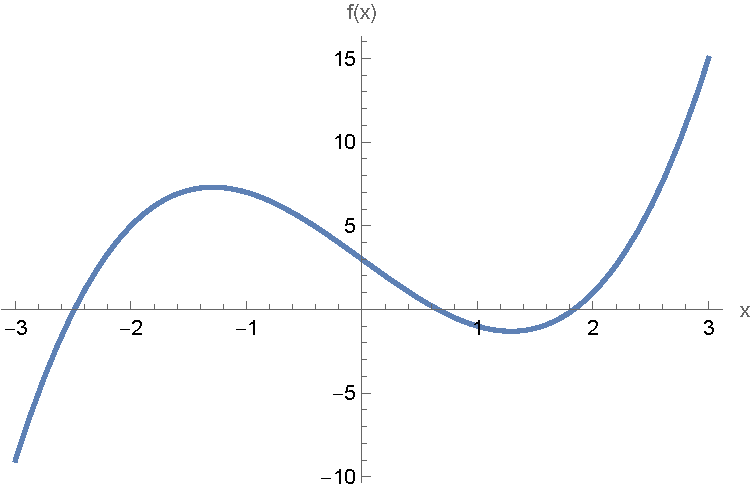
\includegraphics[width=0.6\textwidth]{./Figs/1_plot.pdf}  % 调整图片宽度
    \caption{Plot of $x^3 - 5x + 3 = 0$.}
\end{figure}
发现有两个正根,分别在$[0, 1]$和$[1, 2]$之间,有点好奇二分法的具体实现,便先用Python写一下二分法的动态过程,见\texttt{./Codes/Problem 1/bisection\_visual.py}, 使用\Colorbox{cmdbg}{\lstinline[language=bash]|python -u bisection_visual.py|}运行(需要安装\texttt{matplotlib,numpy}库)。运行后有三个选项,分别是前两个正根的查找与自定义区间查找,可以自行选择。

\texttt{./Codes/Problem 1/}中还有C++实现的二分法、牛顿法、混合法、Brent法与Ridder法,算法实现集成在了\texttt{methods.cpp}中,\texttt{main.cpp}负责封装与交互,\texttt{plotting.cpp}用ASCII绘制了草图,\texttt{functions.cpp}里面存储了本题函数与导数,拎出来是为了便于灵活测试其它函数,\texttt{utils.cpp}里面有两个工具函数,分别负责按照题目三小问的顺序输出结果与对比测试各类方法在三个根上的表现。
使用\Colorbox{cmdbg}{\lstinline[language=bash]|g++ *.cpp -o main|}编译,\Colorbox{cmdbg}{\lstinline[language=bash]|./main|}运行(也有已经编译好的\texttt{main.exe}),按照提示可以选择各类方法或者一起比较,也可以自定义查找区间与容差等参数。
\subsection{伪代码}

\subsection{结果示例}
\begin{figure}[h]
    \centering
    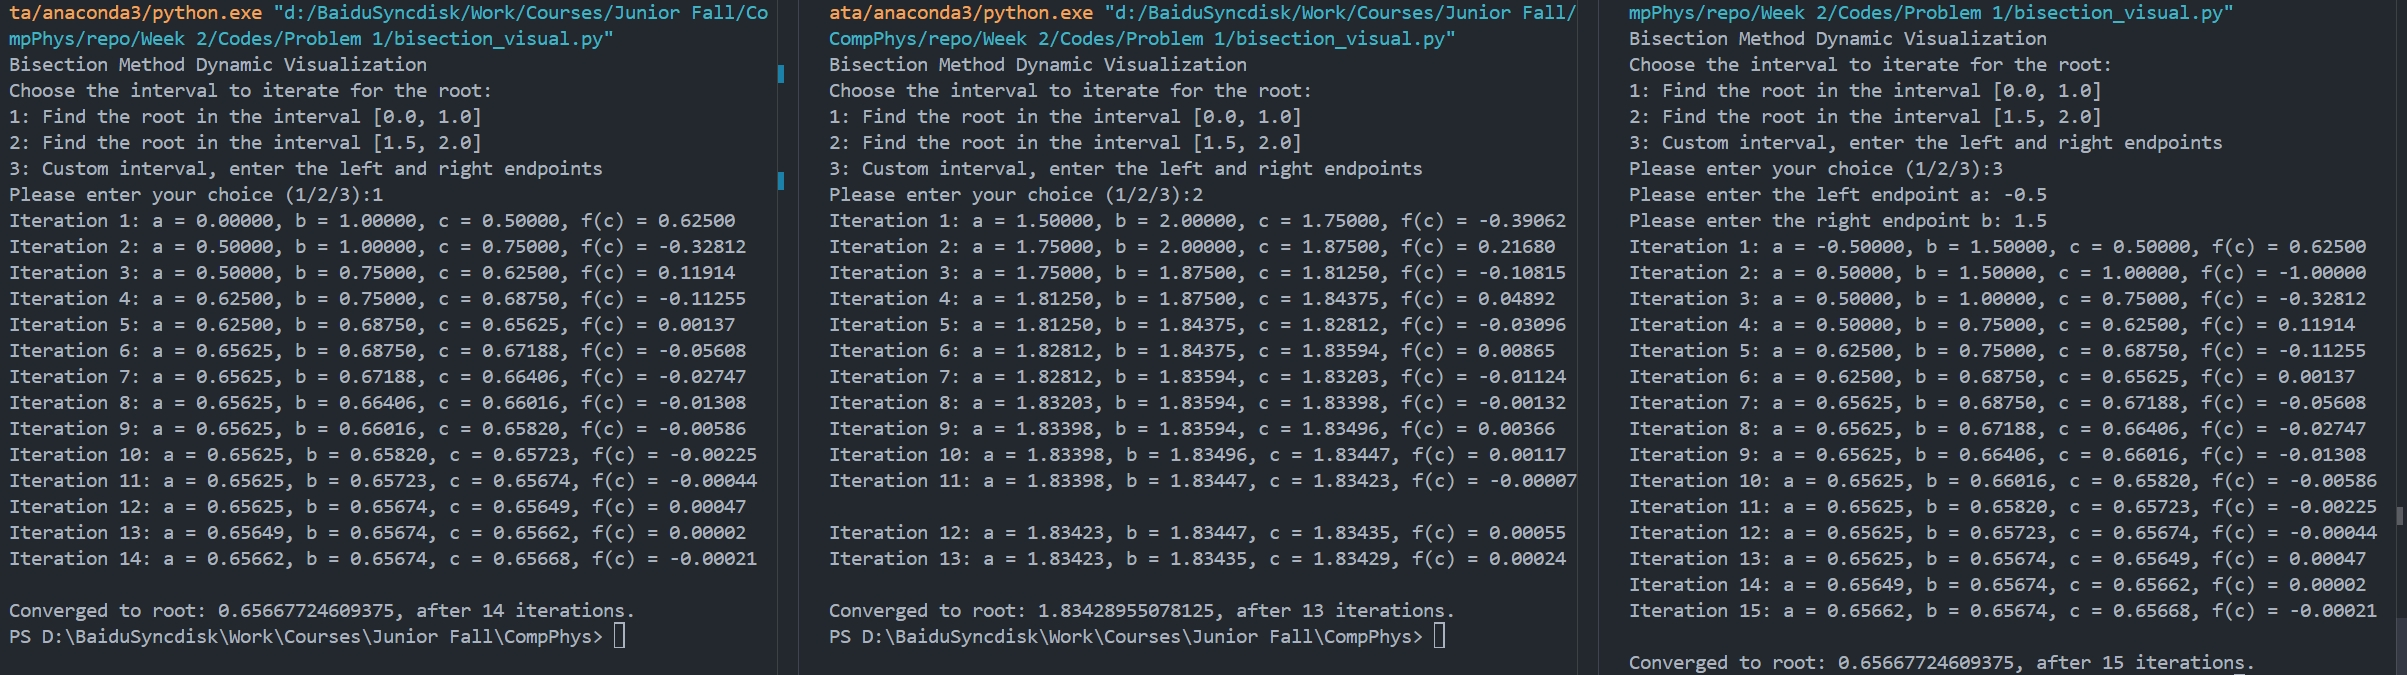
\includegraphics[width=1.0\textwidth]{./Figs/1_bisection.png}
    \caption{\texttt{bisection\_visual.py}三种选项对比}
    \label{fig:1_py_bisection}
\end{figure}

\begin{figure}[H]
    \centering
    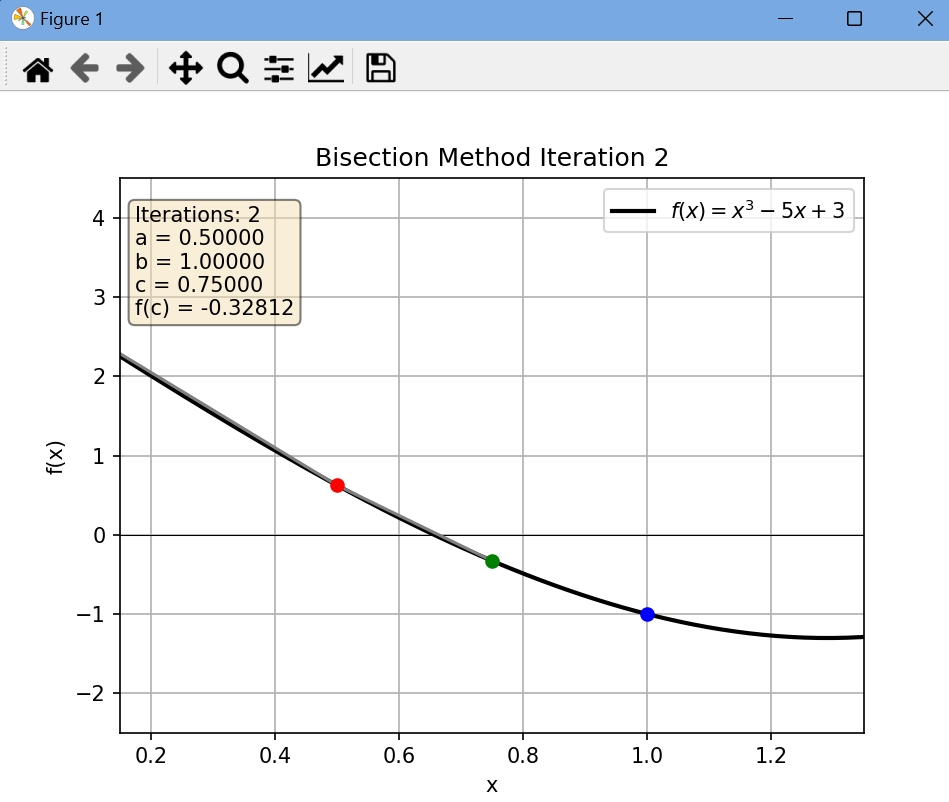
\includegraphics[width=0.6\textwidth]{./Figs/1_animation.png}
    \caption{\texttt{bisection\_visual.py}动画示意}
    \label{fig:1_py_animation}
\end{figure}

\begin{figure}[H]
    \centering
    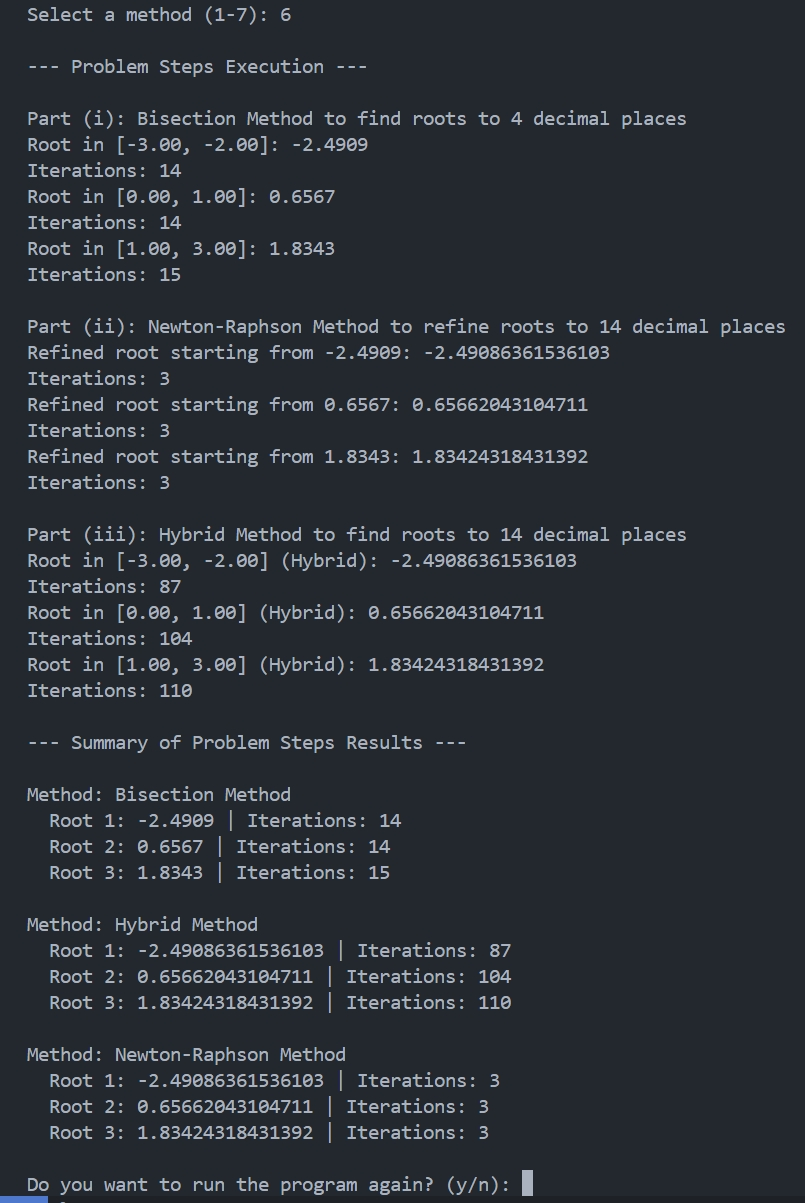
\includegraphics[width=0.7\textwidth]{Figs/1_step.png}
    \caption{\texttt{main.cpp}模式6,按题目顺序尝试三种方法}
    \label{fig:1_cpp_step}
\end{figure}

\begin{figure}[H]
    \centering
    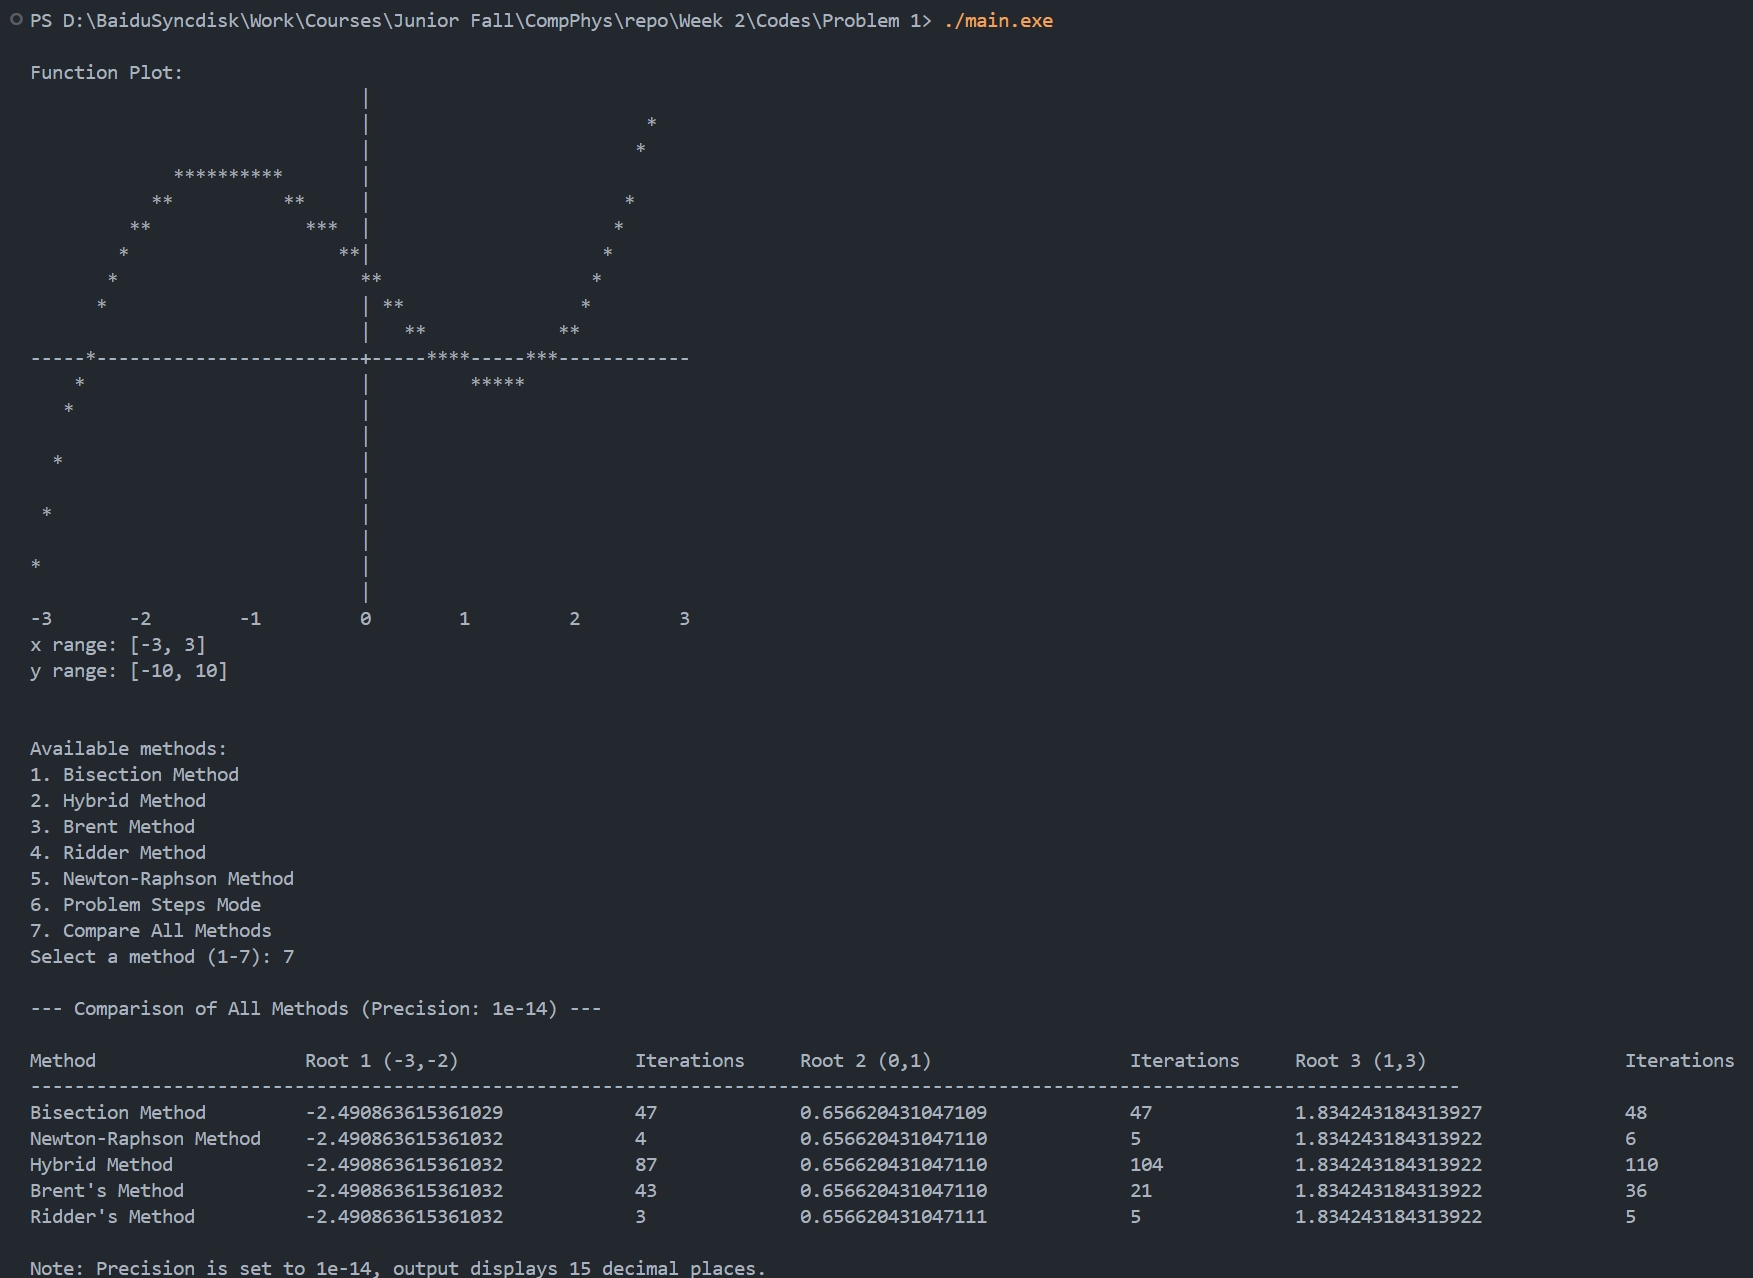
\includegraphics[width=1.0\textwidth]{Figs/1_all.png}
    \caption{\texttt{main.cpp}模式7,对比五种方法}
    \label{fig:1_cpp_all}
\end{figure}
